\documentclass[a4paper]{report}

\usepackage[spanish]{babel}
\usepackage[utf8]{inputenx}
\usepackage[usenames,dvipsnames,svgnames,table]{xcolor}
\usepackage{graphicx}
\usepackage{booktabs}

\newcommand{\executeiffilenewer}[3]{%
  \ifnum\pdfstrcmp{\pdffilemoddate{#1}}%
  {\pdffilemoddate{#2}}>0%
  {\immediate\write18{#3}}\fi%
}

\newcommand{\includegraphics}[1]{%
  \executeiffilenewer{#1.svg}{#1.pdf}%
  {inkscape -z -D --file=#1.svg --export-pdf=#1.pdf --export-latex}%
  \input{#1.pdf_tex}%
}

\begin{document}

\title{Sistema de Información de Redes Productivas\\\textsc{Un mapa de la economía nacional}}
\author{Matías Battocchia \and Gonzalo Flores Kemec}

\maketitle

\section*{Introducción}

% El Gobierno Nacional dentro del marco del Plan Estratégico Industrial 2020 ha asumido el compromiso de promover la industria nacional. Con el fin de aportar a este proceso...

Se presentan las bases de una herramienta original que modela a la industria como una red de redes de valor. Se espera que la misma permita:

\begin{itemize}
  \item Un seguimiento integral de la dinámica productiva sectorial y regional.
  \item El diseño de propuestas y la evaluación de medidas y políticas públicas.
  \item La elaboración de diagnósticos para la toma de decisiones en materia de desarrollo económico.
\end{itemize}

El sistema de información propuesto, en esencia, consiste en representar la estructura de la industria nacional como un \textit{grafo} —definido a continuación—, y en revestir esta representación con información de diversos tipos: económica, social, territorial y tecnológica\footnote{Esta es la primera de las dos ideas fundamentales detrás del sistema.}.

El grafo de la red de cadenas de valor es utilizado por el sistema para \textbf{situar el análisis de datos en el contexto de la red}\footnote{Esta es la segunda idea: Conocer las relaciones subrepticias entre los datos por medio del grafo.}.

\section*{Redes Productivas}

\subsection*{Una definición formal de red}

\begin{figure}[h!]
  \centering
  %\def\svgwidth{\columnwidth}
  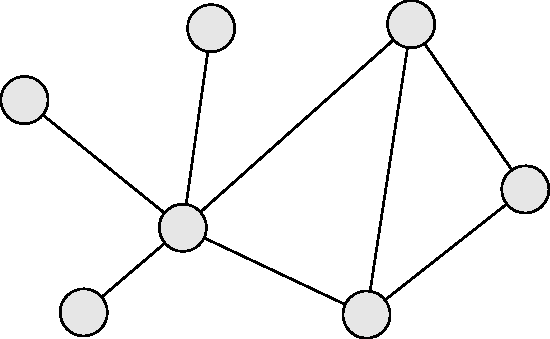
\includegraphics{grafo}
  \caption{Un \textit{grafo} conformado por 7 nodos y 8 relaciones.}
  \label{grafo}
\end{figure}

Los \textit{grafos} son objetos matemáticos que modelan conexiones entre elementos de un conjunto; están compuestos por \textit{nodos} y \textit{relaciones} (figura \ref{grafo}). Muchas estructuras naturales y hechas por el hombre pueden representarse mediante grafos. Con la industria también es factible hacerlo: Los nodos bien pueden ser actividades industriales y las relaciones —\textit{definidas a partir de parejas de nodos}—, pares de actividades inmediatamente conectadas (figura \ref{cadena}).

\begin{figure}[h!]
  \centering
  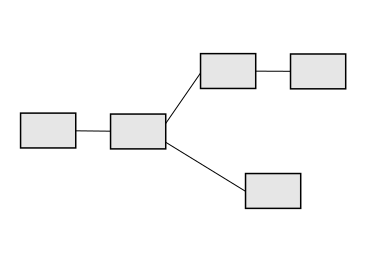
\includegraphics{cadena}
  \caption{Actividades pertenecientes a la cadena de valor del algodón representadas en un grafo.}
  \label{cadena}
\end{figure}

La Teoría de Grafos se ha encargado de estudiar en profundidad estos objetos. Ha desarrollado un sinnúmero de medidas y procedimientos que ponen en evidencia características de los mismos. Mencionaremos ahora algunos de sus conceptos con el fin de ilustrar la teoría en relación al análisis del aparato productivo nacional.

\begin{figure}[h!]
  \centering
  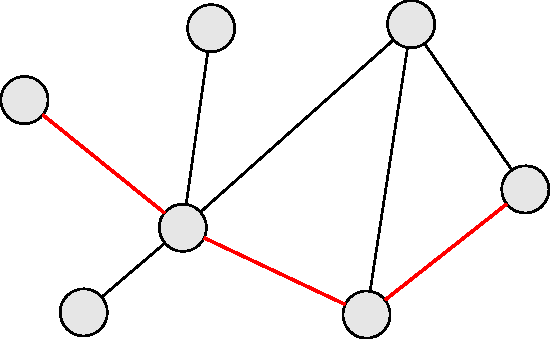
\includegraphics{distancia}
  \caption{La \textit{distancia} del nodo 1 al 5 es igual a 3. Nótese que están unidos por más de un camino, para computarla se eligió uno de los caminos más breves: $1 \rightarrow 4 \rightarrow 7 \rightarrow 5$.}
  \label{distancia}
\end{figure}

Un grafo introduce una noción de \textit{distancia}. Esta se mide en la cantidad de vínculos por los que hay que transitar para ir de un nodo a otro (figura \ref{distancia}). Es común que dos nodos estén conectados por varios posibles caminos; cuando hablamos de distancia nos estamos refiriendo al camino más directo. En el sistema la distancia indica la proximidad entre actividades industriales\footnote{Y la proximidad entre actividades indica el grado de influencia mutua.}.

% La \textit{excentricidad} de un nodo está dada por la distancia a su nodo más lejano en el grafo. Los nodos con alta excentricidad se ubican en la \textbf{periferia} de la red, en cambio los que poseen baja excentricidad conforman el \textbf{centro}.

\begin{figure}[h!]
  \centering
  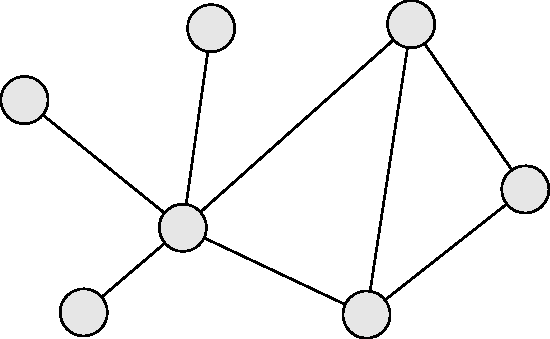
\includegraphics{grados}
  \caption{Se resaltaron las conexiones del nodo 4. Como tiene 5 \textit{primeros vecinos} (nodos 1, 2, 3, 6 y 7) su \textit{grado} es igual a 5.}
  \label{grados}
\end{figure}

Al número de \textit{primeros vecinos} (nodos a distancia 1) que un nodo tiene se le llama \textit{grado} (figura \ref{grados}). Normalmente el grado varía de nodo a nodo. En determinadas redes se encuentran nodos que acaparan significativamente más conexiones que el promedio; a estos se los denomina \textit{hubs}, anglicismo plural para concentrador o conector (figura \ref{hubs}).

\begin{figure}[h!]
  \centering
  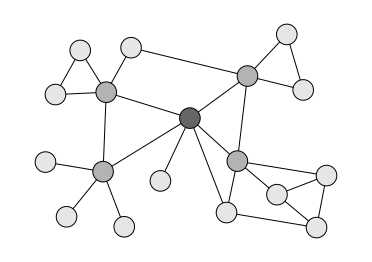
\includegraphics{hubs}
  \caption{Nodos coloreados con tonalidades más obscuras en proporción a su grado. El nodo central se comporta como \textit{concentrador}.}
  \label{hubs}
\end{figure}

Citando un ejemplo, en las redes sociales las personas ``populares'' cumplen el rol de hubs. Aparte de poseer un gran número de contactos —y debido a esto— suelen oficiar de puentes entre distintas comunidades, mejorando la conectividad en la red\footnote{Los hubs son en parte responsables de los \textit{6 grados de separación}. Gracias a ellos ``el mundo es pequeño''.}. El rasgo distintivo de una comunidad es ser un conjunto de personas que se conocen entre sí: nodos agrupados, mutuamente conectados. En el sistema lo más parecido a las comunidades serían las cadenas de valor. Las actividades industriales altamente conectadas que se comportan como nexo entre cadenas, de existir, serían hubs\footnote{Estamos suponiendo que la red industrial es del tipo \textit{scale-free} (posee hubs), aunque probable, podría no ser cierto.}.

Hacemos hincapié en los hubs porque son \textbf{la fortaleza y la debilidad} de las redes que se caracterizan por tenerlos. Como se dijo, hacen un aporte importante a la conectividad de la red; sin embargo el coste de esta ventaja es una red susceptible a fallos ante la anulación o el mal funcionamiento de sus hubs.

Expresar a la industria en el lenguaje de los grafos nos permitirá tomar conocimiento acerca de su topología o forma —particularmente identificar hubs en la misma— y de un gran número de sus propiedades. Las acciones que se deben tomar para impulsar su desarrollo, las prioridades de aplicación, dependen fuertemente de las características de la red.

% Añadir acciones concretas que conviene realizar fundamentadas en este tipo de información.

\subsection*{Más tipos de nodos}

Es posible añadir otras clases de nodos a la representación de la industria para hacerla más realista. Hasta ahora hicimos referencia únicamente a actividades industriales con el fin de allanar la introducción. El sistema de información propuesto en su versión básica agrega a la red de actividades, productos, en una configuración que se conoce como \textit{grafo bipartito}: las actividades se conectan exclusivamente con productos, y los productos con actividades, sin posibilidad de que nodos del mismo tipo se relacionen directamente (figura \ref{bipartito}).

\begin{figure}[h!]
  \centering
  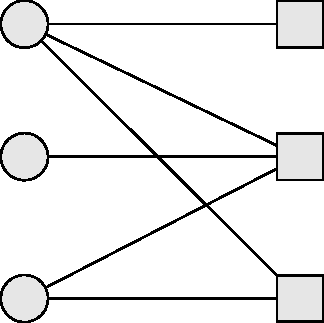
\includegraphics{bipartito}
  \caption{En un grafo \textit{bipartito} nodos de una misma clase no se conectan entre sí. En el diagrama los círculos representan actividades y los cuadrados, productos.}
  \label{bipartito}
\end{figure}

El sistema dispone de una colección de \textbf{actividades} y otra de \textbf{productos}, creadas a partir de la \textsc{Clasificación Internacional Industrial Uniforme}\footnote{Nomenclatura en uso por la AFIP y la ONU para clasificar procesos productivos.} (CIIU) y del \textsc{Sistema Armonizado}\footnote{Nomenclatura ampliamente difundida en el comercio internacional para clasificar manufacturas, en uso por el INDEC y la ONU para elaborar estadísticas.} (SA) respectivamente. Un extracto de estas clasificaciones puede verse en la tabla \ref{extracto}. Sus elementos son las piezas interconectables con las que se construye el grafo de la industria (figura \ref{nomencladores}). Es una característica fundamental del sistema el implementar nomenclaturas utilizadas por organismos nacionales e internacionales para la identificación de los nodos; es lo que posteriormente permite incluir estadísticas con naturalidad, ya que estas se elaboran en base a las clasificaciones mencionadas.

\begin{table}[h]
  \centering
  \begin{tabular}{llr}
    \toprule
    \multicolumn{2}{c}{SA (Productos)} \\
    \midrule
    520100 & Algodón sin cardar ni peinar. \\
    520300 & Algodón cardado o peinado. \\
    520411 & Hilo de coser de algodón, sin acondicionar para la venta al por menor. \\
    \midrule
    \multicolumn{2}{c}{CIIU (Actividades)} \\
    \midrule
    171111 & Desmotado de algodón; preparación de fibras de algodón. \\
    171132 & Fabricación de hilados de algodón y sus mezclas. \\
    171142 & Fabricación de tejidos (telas) planos de algodón y sus mezclas. \\
    \bottomrule
  \end{tabular}
  \caption{Extracto de las nomenclaturas adoptadas por el sistema.}
  \label{extracto}
\end{table}

\begin{figure}[h!]
  \centering
  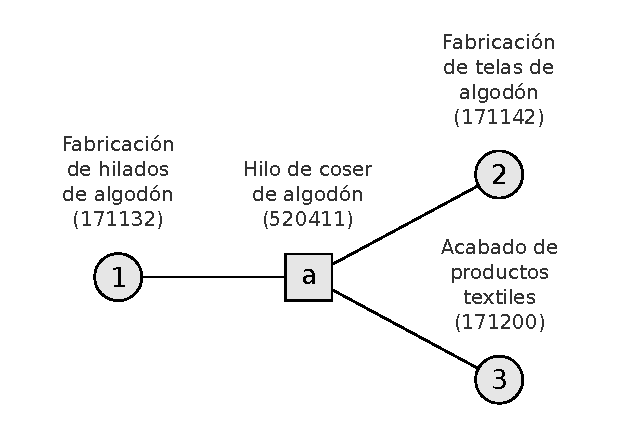
\includegraphics{nomencladores}
  \caption{En el sistema cada nodo del grafo es asociado a un nomenclador que lo identifica. Si se trata de actividades (círculos) estos provienen del CIIU, y si son productos (cuadrados), del SA.}
  \label{nomencladores}
\end{figure}

Las actividades industriales se conectan con productos en \textbf{relación de aprovisionamiento}, discriminando si son insumos, o en \textbf{relación de producción}, sin son manufacturas de la actividad. Este rompecabezas es armado en base a informes sectoriales y regionales existentes, generados por organismos como el Ministerio de Economía y la AFIP.

En el modelo considerado, las actividades son \textbf{procesos de transformación} y los productos \textbf{materia} capaz de ser transformada. A su vez, las relaciones de aprovisionamiento y producción establecen direcciones preferenciales dentro de la red: la materia fluye por caminos que van agregándole valor en cada proceso.

No habíamos recurrido a relaciones direccionadas en la sección anterior. Cuando un grafo las incorpora, se lo conoce como \textit{grafo dirigido} (figura \ref{dirigido}).

\begin{figure}[h!]
  \centering
  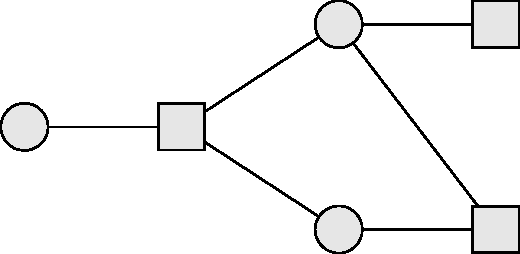
\includegraphics{dirigido}
  \caption{En un grafo \textit{dirigido} las relaciones son direccionadas.}
  \label{dirigido}
\end{figure}

\subsection*{El significado de las estadísticas}

% Series Temporales

La clase de estadísticas a las que el sistema recurre en mayor medida son \textit{series temporales}: secuencias de datos en el tiempo, típicamente espaciados en intervalos temporales uniformes (figura \ref{serie}). En la versión básica del sistema resultan de particular interés la evolución temporal de dos tipos de indicadores: \textbf{cantidades} y \textbf{precios}; combinando estos se pueden calcular otros, como \textbf{precios unitarios}.

\begin{figure}[h!]
  \centering
  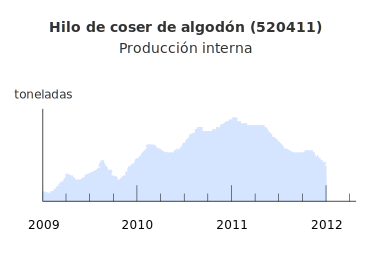
\includegraphics{serie}
  \caption{Ejemplo de \textit{serie temporal}. El artículo va acompañado por su nomenclador.}
  \label{serie}
\end{figure}

% Semántica

Decimos que el grafo de la industria se comporta como un sustrato para las estadísticas. Por un lado, los nodos de la red están identificados por nomencladores, por otro, las estadísticas sobre actividades y productos se elaboran en base a los mismos nomencladores; el sistema entonces adquiere estadísticas y, según los nomencladores, las almacena adjuntándoselas a los nodos (figura \ref{series}). Esta práctica da lugar a una semántica: hace que las series de \textbf{cantidades} aplicadas a \textbf{nodos} signifiquen el \textbf{nivel de actividad} de los procesos o el \textbf{stock} de los productos—dependiendo del tipo de nodo. Asimismo es posible asociar series de \textbf{cantidades} a las \textbf{relaciones} entre nodos; en este caso denotan la \textbf{producción} o el \textbf{consumo} de materia que circula por la red—dependiendo del tipo de relación. Usualmente donde haya un \textbf{flujo de materia} habrá un \textbf{contra-flujo monetario}, plausible de ser descripto por series temporales de \textbf{precios}.

\begin{figure}[h!]
  \centering
  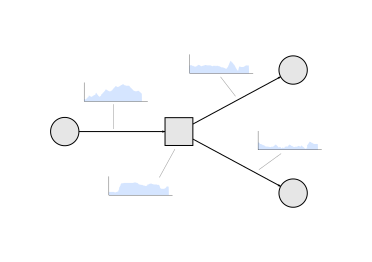
\includegraphics{series}
  \caption{Grafo de la figura \ref{nomencladores} con series temporales asociadas; la que se refiere a la producción es la de la figura \ref{serie}.}
  \label{series}
\end{figure}

% Análisis

Anteriormente dijimos que el grafo introduce una noción de distancia entre nodos. Acabamos de mencionar que podemos asociar series temporales a los nodos. Por lo tanto \textit{el grafo establece una noción de distancia entre series temporales}. Aquí yace el potencial de la herramienta: no es lo mismo analizar estadísticas ``sueltas'' que asentadas en una estructura. El grafo incorpora información de la realidad en el sistema, es un mapa en el que se lee cuáles actividades y productos se afectan directamente (primeros vecinos), cuáles indirectamente a través de un intermediario (segundos vecinos), etcétera.

Las series temporales pueden estudiarse con técnicas provenientes del Análisis de Series Temporales para extraer información significativa. Una de las principales medidas realizables es la \textit{dependencia estadística}\footnote{La dependencia estadística no es condición suficiente para asegurar la dependencia causal entre dos fenómenos.} entre series temporales, llamada \textit{correlación cruzada}. Puede evaluarse por ejemplo en qué grado el aumento o la disminución de la producción de cierto producto influye sobre la de otro y con cuánto retardo temporal.

Lo que el sistema efectúa son correlaciones cruzadas \textit{pesadas} por medio del grafo, es decir que asigna una importancia o un peso a las dependencias estadísticas en función de la distancia de las series\footnote{En este caso el grafo aporta la condición suficiente para interpretar a los resultados estadísticos como dependencias causales.}.

La herramienta puede ser utilizada con fines retrospectivos y prospectivos. Los primeros engloban técnicas de Análisis de Regresión para determinar la calidad de ajuste de modelos teóricos a los datos experimentales y así validar o rechazar teorías. Los segundos recurren a técnicas de Pronóstico de Series Temporales para predecir estados futuros de la industria. También corre simulaciones bajo situaciones hipotéticas para explorar los efectos de distintas políticas industriales.

\subsection*{Aún más posibilidades}

Es posible continuar enriqueciendo el modelo adicionando nuevas clases de nodos\footnote{Este trabajo considera solamente al sector productivo. El financiero se deja para un próximo.}. Cuatro que resultan muy informativas son territorios, labores, mercados y tecnologías. La primera permite procesar datos geográficos para complementar el semblante \textbf{sectorial} con el \textbf{regional}. La segunda agrega una capa de análisis de \textbf{fuerza de trabajo} al mapa\footnote{Las actividades industriales requieren recursos humanos.}. Mercados tenemos externos e internos, son orígenes y destinos de productos\footnote{Los mercados también son una abstracción del comercio, partes de la red desconocidas en detalle.}. Por último, nodos que describen tecnologías existentes, cuyas relaciones con las actividades representan el respectivo grado de transferencia tecnológica\footnote{Los nodos de tecnologías sí se conectan entre sí. Así el sistema modela el árbol de dependencia entre tecnologías.}.

Está dentro de las posibilidades del sistema distinguir subcategorías de productos, tales como bienes de capital, insumos, energía y servicios\footnote{El sistema considera a los servicios como productos intangibles y no-almacenables.}.

El grafo es capaz de asimilar tipos de información de los más diversos. Antes de emprender la construcción de un modelo más complejo, la versión básica —compuesta por actividades y productos— debe madurar. Vale mencionar que el sistema no recurre a datos que el Estado no recabe a través de la AFIP o el INDEC en la actualidad, o tenga la potestad de conseguirlos si se lo propone; en todo caso los obstáculos se hallan en la articulación entre sus propios organismos.

\subsection*{La dinámica de la red}

Hay un tipo de análisis dentro del campo de la Teoría de Grafos que estudia los cambios estructurales de las redes en el tiempo. Las estructuras reales están vivas: los nodos surgen y desaparecen; aún más, las conexiones entre ellos se encuentran en permanente alteración.

De la misma forma en la que una persona que conoce a muchas personas tiene mayores chances de hacerse de un nuevo contacto que quien conoce a muy pocas, una actividad o producto muy conectado tiene altas probabilidades de participar en nuevas relaciones en el futuro. Es el concepto de \textit{conexión preferencial}. Desde el punto de vista de la planificación industrial, predicciones de esta índole estiman demandas en función de relaciones potenciales.

Por otro lado podría utilizarse al sistema para proyectar desarrollos de complejos productivos. Suponiendo que se quiera producir determinado producto íntegramente en el país y que para concretar tal objetivo sea menester establecer nuevos nodos y relaciones, se los detallaría sobre la red vigente para estudiar una forma ordenada de llevar el desarrollo adelante.

\subsection*{Los estratos de agregación}

Hasta ahora se ha hablado de una red agregada. Esta dispone nodos y nomencladores en relación \textit{uno-a-uno}: cada nodo del grafo se corresponde con \textbf{un y sólo un} nomenclador; en otras palabras, diferentes actividades y productos figuran una única vez en la red. El sistema también puede ser orientado hacia el otro extremo, descendiendo al nivel de los agentes económicos.

La red desagregada, en la que se consideran perfiles de empresas, se visualiza como una ``red social'' de empresas. Cada agente agrupa actividades industriales —tal cual figura en su inscripción en la AFIP—, estas actividades producen y consumen productos (figura \ref{perfil}). Nótese que en general las actividades y los productos ahora se repiten en el grafo, debido a las empresas que se dedican a los mismos ramos; en este caso la relación entre nodos y nomencladores es \textit{muchos-a-uno}. Dos empresas tendrán una \textbf{relación comercial} por cada actividad de una que produzca un producto que una actividad de la otra consuma.

\begin{figure}[h!]
  \centering
  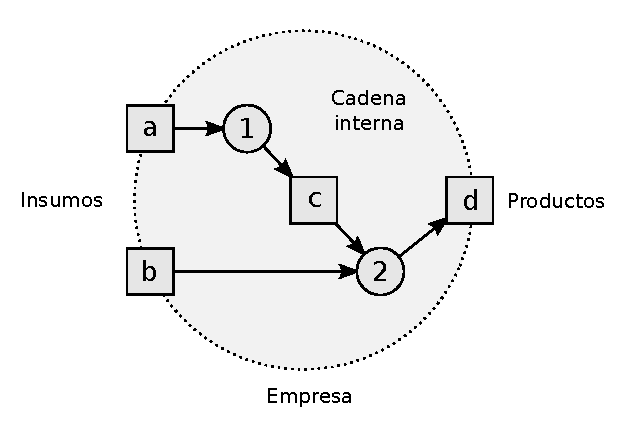
\includegraphics{perfil}
  \caption{Una empresa realiza al menos una actividad (actividad principal). Sus insumos y productos la vinculan con proveedores y clientes.}
  \label{perfil}
\end{figure}

La agregación sucede cuando se integran los datos de las actividades y los productos de las empresas, discriminando por nomenclador. Este procedimiento genera la estructura de la red agregada, que emerge del comportamiento de los agentes (figura \ref{estratos}).

%La intensidad de las relaciones es función de la cantidad de tales intercambios.

\begin{figure}[h!]
  \centering
  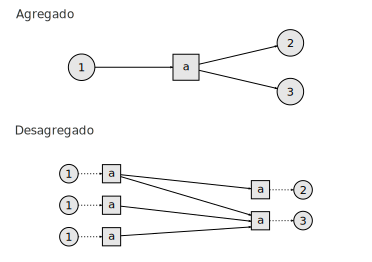
\includegraphics{estratos}
  \caption{En la red desagregada tres empresas que realizan la \textbf{actividad 1} proveen del \textbf{producto a} a una empresa que se dedica a la \textbf{actividad 2} y a otra que trabaja la \textbf{actividad 3}. La red agregada lo refleja conectando al producto con todas las actividades en las que este participa.}
  \label{estratos}
\end{figure}

Las actividades de las empresas pueden asociarse a localidades geográficas. El plano desagregado le confiere especial interés a la información territorial, permitiendo analizar y optimizar la logística de cargas. Los distintos estratos de agregación se enfocan en provincias y regiones para trabajar sobre estrategias coyunturales. Permitiéndonos pensar en grande, el sistema de información serviría para planificar la integración productiva del MERCOSUR de ser usado por el resto de los países socios.

Otra funcionalidad del sistema es la de ser usado por los agentes económicos para obtener información personalizada de su contexto productivo, buscar clientes y proveedores, administrar operaciones comerciales, recibir sugerencias de inversión. Los agentes suministran información personal\footnote{Nos referimos a personas en general: físicas y jurídicas.} a cambio de reportes personalizados; el sistema luego la incluye en su base de datos.

En comparación con los datos agregados, los desagregados son más costosos de recopilar. Los primeros suelen publicarse, los segundos usualmente son confidenciales. Lo expuesto en el párrafo anterior es un recurso para conseguirlos: los datos personales son el punto de partida de las devoluciones personalizadas. Otro instrumento —con particular potencial para trazar la red comercial— son las facturas electrónicas.

Si bien la idea es que los datos desagregados sean volcados en los perfiles de empresas y que sea el propio sistema quien los agregue, inicialmente este se nutrirá de información agregada—a causa de la dificultad mencionada. La adquisición de datos desagregados se implementará en etapas posteriores de su desarrollo.

Realizar un seguimiento de todas las empresas del país es sin duda una tarea complicada. Existen posibilidades de intentar una aproximación: que el sistema sea consciente aunque sea de las grandes empresas, una cifra más asible que si se tratara del total; después de todo el \textit{Principio de Pareto}\footnote{Vagamente enunciado: El 20\% de los agentes genera el 80\% de la riqueza.} nos indica que este grupo reducido de empresas controla la mayor porción del mercado. Esto alcanzaría para practicar algunas estimaciones.

\subsection*{Una base de datos pública y abierta}

El sistema organiza y almacena una gran cantidad de datos para su funcionamiento. Tanto los datos crudos como los procesados (siempre que sean considerados públicos) podrán ser consultados y/o descargados para su uso general por medio de la \textit{interfaz web} del sistema, mientras que al mismo tiempo estarían disponibles a través de un \textit{servicio web} para ser accedidos por otros sistemas informáticos cómodamente.

En general el acceso a datos sobre el país en la actualidad es restringido, principalmente porque no se encuentran publicados o no lo están en un formato apto para máquinas: informes en \textsc{PDF}, \textsc{DOC}, \textsc{XLS}, fáciles de comprender para el humano pero costosos para la computadora. Por esta razón creemos que el sistema puede ser un aporte sin precedentes en el campo de los \textbf{datos abiertos}. Terceros —especialmente la Academia— podrían aprovecharlo para contrastar modelos económicos, crear indicadores, estudiar políticas, e inclusive proponer mejoras al mismo sistema\footnote{Este uso rememora a la filosofía del software libre.}, entre otros usos.

\section*{Conclusiones}

% planificación económica
% desarrollo provincial y regional
% desarrollo sectorial
% exportación/importación
% logística de cargas
% coyuntura regional (interno)
% inserción comercial (externo)

La conjunción de la Teoría de Grafos y el Análisis de Series Temporales aplicada al diseño de políticas de desarrollo industrial promete superar a los análisis económicos convencionales.

La herramienta propuesta modela la industria para generar información sistematizada relevante para la planificación económica, el desarrollo sectorial y regional, la integración productiva, la inserción comercial en mercados externos, la substitución de importaciones, la logística de cargas.

La herramienta automatiza diagnósticos que indican y \textit{priorizan} políticas económicas para fortalecer la industria, e informa sobre sus resultados.

Es necesaria una integración transversal de los sistemas de información de los diversos organismos del Estado para producir políticas públicas de segunda generación.

\end{document}
